\section{Experimental Evaluation}
\label{sec:experiment}

% NOTE: every figure in this section is a native pgfplots chart drawn by LaTeX
% in Overleaf -- one series per individual dataset, with inline coordinates and
% NO external image files, so this .tex is fully self-contained.
% The ONLY requirement is in the MAIN document preamble:
%   \usepackage{pgfplots}\usepackage{subcaption}\pgfplotsset{compat=1.17}
% pgfplots dataset colors (used by the per-dataset figures below):
\definecolor{c0}{HTML}{1F77B4}\definecolor{c1}{HTML}{FF7F0E}\definecolor{c2}{HTML}{2CA02C}\definecolor{c3}{HTML}{D62728}\definecolor{c4}{HTML}{9467BD}\definecolor{c5}{HTML}{8C564B}

We evaluate clamped $w$-event differential privacy with $P$-allocation on six real-world IoT datasets that span the three motivating scenarios of Section~\ref{sec:inference-attacks} (traffic, smart-meter energy, wearable health) plus three additional benchmarks covering urban air quality, urban mobility, and industrial manufacturing. The goals of the evaluation are:
\begin{enumerate}
% \item \textbf{Algorithm~\ref{alg:greedy-tune} (greedy hill-climb over $P$).} 
\item \textbf{Window size $w$.} Verify the linear dependence of the Laplace scale $\lambda_\tau = \Delta_f\,w/\epsilon$ (Theorem~\ref{thm:s-sensitive-budget}) on $w$, holding $P$, $\epsilon$, and the allocation strategy fixed.
\item \textbf{Privacy budget $\epsilon$.} Verify the inverse dependence of $\lambda_\tau$ on $\epsilon$ (again Theorem~\ref{thm:s-sensitive-budget}), holding $P$, $w$, and the allocation strategy fixed.
\item \textbf{Ablation study} Verify the independent impacts of each of our utility hyper parameters on downstream subscriber utility given publisher privacy constraints
\item \textbf{Overhead Comparison} Compare the throughput and latency impacts of our model versus an classic publish-subscribe broker
\item \textbf{Induced Latency} Compare the delay, $k_{ext}$ invocations across datasets to determine how much latency our model adds to various topic hierarchies
\item \textbf{Average Case Utility} Empirically measure the average case of our models utility under normal publisher churn
\end{enumerate}
Each experiment isolates a single axis of the hyperparameter space (Section~\ref{sec:tuning}) so the effect on utility is unambiguous, complementing the full parameter sweep in \texttt{sweep} and the motivating Figure~\ref{fig:distortion-vs-scope} from Section~\ref{sec:streaming-gap}.

\subsection{Implementation}
\label{sec:impl}

We implement the privacy mechanism as a plugin to an MQTT broker (\texttt{plugin.py}). The full source, experiment harness, and dataset loaders are available at \url{https://github.com/DIPrLab/PubSubPrivacy}. The plugin interposes between publishers and subscribers: it subscribes to all raw topics under a configurable prefix (e.g., \texttt{factory/raw/\#}), buffers incoming messages within each discrete timestamp interval $\Delta t$ starting at $t_\tau^{\text{start}}$, clamps each payload to its publisher-specific interval $[a_p, b_p]$ (Definition~\ref{def:clamp-range}), computes the per-topic clamped aggregation $\gamma_\tau = f(D_\tau)$ (default mean), applies the $w$-event Laplace mechanism with scale $\Delta_f/\epsilon_\tau$, and publishes on the subscriber's protected topic exactly one pair $(\hat{\gamma} _\tau, t_\tau^{\text{start}})$. The broker-internal quantities $n_\tau$, $\mathrm{scope}(\tau)$, $\epsilon_\tau$, $\lambda_\tau$, and $\tau$ itself are not transmitted. We build the topic hierarchies based on standard publish subscribe benchmarking on the same datasets \cite{CHRISTIAN}.


At each interval $\tau$, the broker collects $\{\tilde{x}_{p,\tau} : p \in \mathcal{P}_\tau\}$, computes $\gamma_\tau = f(D_\tau)$ and $n_\tau = |\mathcal{P}_\tau|$, derives the data-independent sensitivity $\Delta_f$ from $R$ and $n_\tau$ (Table~\ref{tab:sensitivity-defaults}), and hands everything to the allocation strategy. Notably, $P$ does not appear in the noise scale; it enters only through the strategy's scheduling decision. The per-element budget $\epsilon_\tau$ returned by the strategy is clipped to the remaining window budget $\epsilon - \sum_{j=\tau-w+1}^{\tau-1} \epsilon_j$, and the release uses Laplace noise of scale $\Delta_f/\epsilon_\tau$.

\begin{algorithm}[t]
\caption{Per-element release at interval $\tau$ (wall-clock start $t_\tau^{\text{start}}$)}\label{alg:release}
\begin{algorithmic}[1]
\Require Clamped aggregate $\gamma_\tau = f(D_\tau)$, multiplicity $n_\tau$,
clamp $R$, aggregation $f$ with sensitivity $\Delta_f = \Delta_f(R, n_\tau)$,
DP budget $\epsilon$, window $w$, strategy $\mathcal{A}$, last released noisy aggregate $\hat{\gamma} ^{\text{last-rel}}$, interval start $t_\tau^{\text{start}}$
\Ensure Delivered pair $(\hat{\gamma} _\tau, t_\tau^{\text{start}})$
\State $(\epsilon_{\tau,1},\ \epsilon_{\tau,2},\ \textit{defer}) \gets \mathcal{A}.\textsc{Allocate}(\tau, \gamma_\tau, n_\tau, \hat{\gamma} ^{\text{last-rel}})$
  \Comment{$\epsilon_{\tau,1}$: dissimilarity charge (BD/BA only); $\epsilon_{\tau,2}$: publication charge}
\State $\epsilon_\tau \gets \min\!\bigl(\epsilon_{\tau,1} + \epsilon_{\tau,2},\; \epsilon - \sum_{j=\tau-w+1}^{\tau-1} \epsilon_j\bigr)$
  \Comment{Enforce window budget~\eqref{eq:budget-thm} on the total per-timestamp charge}
\State $\epsilon_{\tau,2} \gets \max\!\bigl(0,\; \epsilon_\tau - \epsilon_{\tau,1}\bigr)$
  \Comment{Re-derive publication share after the clip; $\epsilon_{\tau,1}$ is already spent}
\If{$\textit{defer}$ \textbf{or} $\epsilon_{\tau,2} \le 0$}
  \State $\hat{\gamma} _\tau \gets \hat{\gamma} ^{\text{last-rel}}$; record $\epsilon_\tau$ in sliding window
  \State \Return $(\hat{\gamma} _\tau, t_\tau^{\text{start}})$
\EndIf
\State $\lambda_\tau \gets \Delta_f / \epsilon_{\tau,2}$ \Comment{$\Delta_f$ depends only on public $R$ and $n_\tau$}
\State $\hat{\gamma} _\tau \gets \gamma_\tau + \mathrm{Lap}(\lambda_\tau)$
\State Record $\epsilon_\tau$ in sliding window; update $\hat{\gamma} ^{\text{last-rel}} \gets \hat{\gamma} _\tau$
\State \Return $(\hat{\gamma} _\tau, t_\tau^{\text{start}})$ \Comment{Only the aggregate and interval start are delivered}
\end{algorithmic}
\end{algorithm}


We implement the four budget-allocation strategies from Kellaris et al.~\cite{kellaris2014} (Uniform, Sample, Budget Distribution, Budget Absorption), our new $n$-weighted allocation (Section~\ref{sec:n-weighted}), and three of them composed through the $P$-gated wrapper ($P$-gated Uniform, $P$-gated Sample, $P$-gated BA; Section~\ref{sec:p-allocation}). Each strategy returns a triple $(\epsilon_{\tau,1}, \epsilon_{\tau,2}, \textit{defer})$ to Algorithm~\ref{alg:release}, where $\epsilon_{\tau,1}$ is the dissimilarity-test charge spent inside the strategy (zero for strategies without value-similarity skipping) and $\epsilon_{\tau,2}$ is the publication share reserved for the noisy release. The $P$-gated wrapper first invokes the clamp-compatible greedy scope walk (Algorithm~\ref{alg:greedy-scope}) to find the release scope; if no ancestor meets $P$ the timestamp is deferred, otherwise the inner strategy is invoked on the scope-scoped $n_\tau$. Because $n_\tau$ and the clamp intervals are public under the neighboring relation, both gating and $n$-weighting consume no privacy budget and do not enter the Laplace scale.

\begin{algorithm*}[t]
\caption{Budget-allocation strategies. Every procedure returns the triple $(\epsilon_{\tau,1}, \epsilon_{\tau,2}, \textit{defer})$ consumed by Algorithm~\ref{alg:release}; $\epsilon_{\tau,1}$ is the dissimilarity charge already spent inside the strategy, $\epsilon_{\tau,2}$ is the publication budget reserved for the noisy release, and \textit{defer} signals whether to repeat the previous output.}\label{alg:strategies}
\begin{algorithmic}[1]
\Procedure{Uniform.Allocate}{$\tau, \gamma_\tau, n_\tau, \hat{\gamma} ^{\text{last-rel}}$}
  \State \Return $(0,\; \epsilon / w,\; \textit{false})$
\EndProcedure
\Statex
\Procedure{Sample.Allocate}{$\tau, \gamma_\tau, n_\tau, \hat{\gamma} ^{\text{last-rel}}$}
  \If{$(\tau - 1) \bmod w = 0$} \Comment{Equivalent to $\tau \bmod w = 1$ for $w \ge 2$; also fires every $\tau$ when $w = 1$ (event-level privacy)}
    \State \Return $(0,\; \epsilon,\; \textit{false})$
  \Else
    \State \Return $(0,\; 0,\; \textit{true})$
  \EndIf
\EndProcedure
\Statex
\Procedure{BudgetDistribution.Allocate}{$\tau, \gamma_\tau, n_\tau, \hat{\gamma} ^{\text{last-rel}}$}
  \Comment{Two-stage budget (Kellaris et al.~\cite{kellaris2014}, Sec.~4.2): Stage~1 is a noisy dissimilarity test against the last noisy release $\hat{\gamma} ^{\text{last-rel}}$ (post-processing); Stage~2 forward-distributes the unspent publication share on a skip.}
  \State $\epsilon_{\tau,1} \gets \epsilon / (2w)$ \Comment{Fixed Stage-1 dissimilarity charge}
  \State $\widetilde{\mathrm{dis}}_\tau \gets |\gamma_\tau - \hat{\gamma} ^{\text{last-rel}}| + \mathrm{Lap}\!\bigl(\Delta_f / \epsilon_{\tau,1}\bigr)$
    \Comment{Sensitivity of $|\gamma_\tau - \hat{\gamma} ^{\text{last-rel}}|$ is $\Delta_f$; $\hat{\gamma} ^{\text{last-rel}}$ is fixed across DP-neighbors}
  \State $\epsilon_{\tau,2}^{\text{nom}} \gets \epsilon / (2w) + b_{\text{fwd}}[\tau]$
    \Comment{Stage-2 publication base $+$ forwarded shares from prior skips}
  \If{$\widetilde{\mathrm{dis}}_\tau < \theta \cdot R$} \Comment{$\theta = 0.1$; the noised aggregate is close enough to repeat}
    \State For $j = 1, \ldots, w-1$: $b_{\text{fwd}}[\tau + j] \mathrel{+}= \dfrac{\epsilon/(2w)}{w-1}$
      \Comment{Forward only the base publication share, not the accumulated $b_{\text{fwd}}[\tau]$, so a single original share never propagates more than one hop}
    \State \Return $(\epsilon_{\tau,1},\; 0,\; \textit{true})$ \Comment{Skip; only Stage-1 budget is spent}
  \Else
    \State $b_{\text{fwd}}[\tau] \gets 0$
    \State \Return $(\epsilon_{\tau,1},\; \epsilon_{\tau,2}^{\text{nom}},\; \textit{false})$
  \EndIf
\EndProcedure
\Statex
\Procedure{BudgetAbsorption.Allocate}{$\tau, \gamma_\tau, n_\tau, \hat{\gamma} ^{\text{last-rel}}$}
  \Comment{Two-stage budget (Kellaris et al.~\cite{kellaris2014}, Sec.~4.3 and Fig.~4 lines~5--6): Stage~1 noisy dissimilarity test as in BD; Stage~2 absorbs the publication shares of skipped timestamps into the next release and nullifies the same number of following timestamps so the window invariant $\sum \epsilon_{\tau,2} \le \epsilon/2$ holds pointwise rather than only via the cap of Algorithm~\ref{alg:release}.}
  \Comment{State carried across taus: $b_{\mathrm{absorbed}}$ counts skipped publication shares waiting to be absorbed; $b_{\text{nullify}}$ counts taus whose Stage~2 share is forced to null after a previous absorbing release.}
  \State $\epsilon_{\tau,1} \gets \epsilon / (2w)$
  \State $\widetilde{\mathrm{dis}}_\tau \gets |\gamma_\tau - \hat{\gamma} ^{\text{last-rel}}| + \mathrm{Lap}\!\bigl(\Delta_f / \epsilon_{\tau,1}\bigr)$
  \If{$b_{\text{nullify}} > 0$}
    \Comment{Nullification: skip Stage~2 by fiat regardless of the dissimilarity outcome}
    \State $b_{\text{nullify}} \gets b_{\text{nullify}} - 1$
    \State \Return $(\epsilon_{\tau,1},\; 0,\; \textit{true})$
  \EndIf
  \If{$\widetilde{\mathrm{dis}}_\tau < \theta \cdot R$ \textbf{and} $\hat{\gamma} ^{\text{last-rel}}$ defined} \Comment{$\theta = 0.1$}
    \State $b_{\mathrm{absorbed}} \gets \min\!\bigl(b_{\mathrm{absorbed}} + \epsilon/(2w),\; (w-1)\,\epsilon/(2w)\bigr)$
      \Comment{Only the publication share accrues; cap absorption depth at $w-1$ shares}
    \State \Return $(\epsilon_{\tau,1},\; 0,\; \textit{true})$
  \EndIf
  \State $k \gets 1 + b_{\mathrm{absorbed}} \cdot 2w / \epsilon$
    \Comment{Number of base shares (1 fresh $+$ previously absorbed) consumed at this release}
  \State $\epsilon_{\tau,2} \gets k \cdot \epsilon/(2w)$
  \State $b_{\text{nullify}} \gets k - 1$;\quad $b_{\mathrm{absorbed}} \gets 0$
    \Comment{Force the next $k-1$ taus' Stage~2 to null so $\sum_\tau \epsilon_{\tau,2} \le \epsilon/2$ holds in every window of size $w$}
  \State \Return $(\epsilon_{\tau,1},\; \epsilon_{\tau,2},\; \textit{false})$
\EndProcedure
\Statex
\Procedure{NWeighted.Allocate}{$\tau, \gamma_\tau, n_\tau, \hat{\gamma} ^{\text{last-rel}}$}
  \Comment{Section~\ref{sec:n-weighted}, weights $\epsilon$ by $n_\tau$}
  \State Let $Q$ be a sliding deque of the last $w-1$ past logical-timestamp counts
  \Comment{Current $n_\tau$ is the $w$-th entry, added to the denominator below}
  \If{$|Q| < w - 1$}
    \State \Return $(0,\; \epsilon / w,\; \textit{false})$ \Comment{Warm-up: Uniform until window is full}
  \EndIf
  \State $S \gets n_\tau + \sum_{j \in Q} n_j$ \Comment{Sum of $w$ multiplicities in the window}
  \State Append $n_\tau$ to $Q$ (after the release)
  \State \Return $(0,\; \epsilon \cdot n_\tau / S,\; \textit{false})$ \Comment{See Eq.~\eqref{eq:n-weighted}}
\EndProcedure
\Statex
\Procedure{$P$-Gated.Allocate}{$\tau, \gamma_\tau, n_\tau, \hat{\gamma} ^{\text{last-rel}}$;\ inner $\mathcal{A}$}
  \State $(\mathrm{scope}, n_\tau) \gets \textsc{GreedyScopeWalk}(t_{\text{sub}}, \mathcal{P}_\tau, P, R)$
    \Comment{Algorithm~\ref{alg:greedy-scope}}
  \If{$\mathrm{scope} = \bot$}
    \State \Return $(0,\; 0,\; \textit{true})$ \Comment{Defer (no clamp-compatible ancestor has $\geq P$)}
  \Else
    \State \Return $\mathcal{A}.\textsc{Allocate}(\tau, \gamma_\tau, n_\tau, \hat{\gamma} ^{\text{last-rel}})$
      \Comment{Inner strategy keeps its own $(\epsilon_{\tau,1},\epsilon_{\tau,2})$ semantics}
  \EndIf
\EndProcedure
\end{algorithmic}
\end{algorithm*}


The plugin runs as a separate MQTT client connected to the same broker as the publishers and subscribers. It subscribes to all topics under a configurable raw prefix, maintaining a per-topic buffer that maps publisher identifiers to their most recent clamped payload within the current timestamp interval. A periodic timer fires every $\Delta t$ seconds; at each tick the plugin executes Algorithm~\ref{alg:release} for every active topic, publishes the result together with the wall-clock interval start time on the corresponding protected topic, and clears the buffer. When $n_\tau < P$ at the leaf scope and extensions are available, the plugin first applies the adaptive interval extension of Section~\ref{sec:dynamic-timestamp} (up to $K_{\text{ext}}$ extensions of $\Delta t$, giving a worst-case wait $T_{\max} = K_{\text{ext}}\!\cdot\!\Delta t$); only then does it fall back to the greedy clamp-compatible scope walk of Algorithm~\ref{alg:greedy-scope}. Each topic maintains an independent \texttt{StreamState} comprising the sliding budget window of size $w$, the last noisy release $\hat{\gamma} ^{\text{last-rel}}$ used by the dissimilarity sub-mechanism $M_{i,1}$, the BD forward-distribution buffer $b_{\text{fwd}}$, and the BA bookkeeping pair $(b_{\mathrm{absorbed}}, b_{\text{nullify}})$ that drives absorption and nullification. The plugin is stateless across topics: no cross-topic information is used, so the $w$-event $\epsilon$ guarantee holds independently per subscription.

\subsection{Datasets and Topic Hierarchies}
\label{sec:datasets}

Table~\ref{tab:datasets} summarizes the six publicly available IoT datasets we evaluate on. Each dataset is ingested by \texttt{data\_streams.py}, which registers it in a \texttt{DATASETS} dictionary binding the raw CSV(s) to (i) a per-sensor stream builder that resamples raw rows into the pair $(\gamma_\tau, n_\tau)$, (ii) a per-publisher table used for the per-topic experiments, (iii) the operator-declared static clamp intervals $[a_p, b_p]$ of Option~A (Definition~\ref{def:clamp-range}), (iv) a public fallback bound $M$ for the Option~B DP-released calibration, and (v) the normative MQTT topic hierarchy on which the mechanism publishes.

\begin{table*}[t]
\centering
\footnotesize
\caption{Real-world IoT datasets used in the evaluation. \emph{All six datasets are real, public IoT data --- no synthetic measurements are used anywhere.} The \emph{Pub.} column indicates whether the publisher identity is a genuine per-row entity in the source (\textbf{R}eal) or a structural grouping we synthesize from data that is present but lacks an explicit publisher column (\textbf{S}ynth; see \S\ref{sec:pub-construction}). $|\mathcal{P}|$ is the number of distinct publishers; $\Delta t$ is the base wall-clock timestamp interval; $h$ is the depth of the topic hierarchy (number of levels). The topic trees themselves are not shipped with the source CSVs --- we \emph{construct} them per dataset following the PSMark/PerCom domain conventions (\S\ref{sec:topic-construction}); $R$ per sensor is computed from the Option~A static clamp intervals declared in \texttt{DATASETS}.}\label{tab:datasets}
\begin{tabular}{lllrclrl}
\toprule
Dataset (key) & Domain & Source & $|\mathcal{P}|$ & Pub. & Sensors evaluated & $h$ & Topic hierarchy (constructed) \\
\midrule
\texttt{energy}        & Smart-building energy & MCEC-Thai public CSV         & 12 circuits     & R & power (kW), voltage, current               & 4 & \texttt{energy/building01/\{CT\}/\{metric\}} \\
\texttt{traffic}       & Intersection traffic  & Colorado Springs public feed & 4--8 sensors    & R & speed, object count                        & 5 & \texttt{traffic/intersection01/\{kind\}/\{id\}/\{metric\}} \\
\texttt{wearable}      & Wearable health       & Kaggle (dcsavinod)           & 10 devices      & R & heart rate, steps, temperature, calories   & 4 & \texttt{health/\{hospital\}/\{device\}/\{metric\}} \\
\texttt{pune}          & Urban air quality     & Kaggle (akshman)             & 10 stations     & R & PM10, PM2.5, humidity, sound, ozone        & 4 & \texttt{air\_quality/pune/\{station\}/\{pollutant\}} \\
\texttt{mobility}      & Smart mobility        & Kaggle (ziya07)              & 16 cells (4$\times$4) & S & speed, vehicle count, occupancy, emission & 5 & \texttt{mobility/nyc/\{quadrant\}/\{cell\}/\{metric\}} \\
\texttt{manufacturing} & Industrial process    & Kaggle (programmer3)         & 10 sub-machines & S & temperature, speed, vibration, quality     & 5 & \texttt{factory/line1/\{station\}/\{machine\}/\{sensor\}} \\
\bottomrule
\end{tabular}
\end{table*}


For each dataset and each registered sensor, the loader resamples the raw rows into a discrete-time stream with base interval $\Delta t$. At each logical timestamp $\tau$ we have (i) the clamped aggregate $\gamma_\tau = \mathrm{mean}\{\tilde{x}_{p,\tau} : p \in \mathcal{P}_\tau\}$, and (ii) the multiplicity $n_\tau = |\mathcal{P}_\tau|$. Each per-publisher reading is mapped to an MQTT topic under the \texttt{topic\_root} of Table~\ref{tab:datasets}. The topic-hierarchy walk of Section~\ref{sec:subscription-rewriting} operates on these live topic trees during every $P$-gated release.

\subsubsection{Real vs.\ synthesized publishers}
\label{sec:pub-construction}
All six datasets are real public IoT measurements; the only modeling choice is how the publisher set $\mathcal{P}$ is recovered. Four datasets (\texttt{energy}, \texttt{traffic}, \texttt{wearable}, \texttt{pune}) carry an explicit per-row sender, so each publisher is a genuine physical entity: a metered circuit (\texttt{CT1}--\texttt{CT17}), a radar/lidar unit (\texttt{EVO\_RADAR\_1}--\texttt{4}, \texttt{OS1\_LIDAR\_1}--\texttt{2}), a wearable device (\texttt{Device\_1}--\texttt{10}), or a fixed monitoring station. The remaining two (\texttt{mobility}, \texttt{manufacturing}) ship as time-indexed tables \emph{without} a per-row publisher column; for those we synthesize publisher IDs from structure that is genuinely present in the data --- a $4\times4$ \texttt{(lat,lon)} quantile grid of virtual intersection sensors for \texttt{mobility}, and the minute-index within each $\Delta t$ bucket as sub-publishers \texttt{sub\_0}--\texttt{sub\_9} for the single-machine \texttt{manufacturing} feed. These two (marked \textbf{S} in Table~\ref{tab:datasets}) exercise the $\Delta t$ discretization faithfully but are an acknowledged limitation: a different binning would yield a different $\mathcal{P}$.

\subsubsection{Topic-hierarchy construction}
\label{sec:topic-construction}
The source CSVs are flat tables; they do \emph{not} ship MQTT topic trees, so we construct one per dataset. We follow PSMark~\cite{CHRISTIAN}, the distributed publish/subscribe IoT benchmark whose device specification defines, per domain, the device types, per-device metrics, and an edge-server/deployment grouping (e.g.\ factory floors and stations, regional hospitals, smart-city sub-domains). PSMark prescribes the \emph{structure} but not literal topic strings, so we realize it as \texttt{<domain>/<edge-server-or-grouping>/<device>/<metric>} and populate the device/metric levels from each dataset's real entities. This yields realistic multi-level trees of depth $h\!\in\![4,5]$ (Table~\ref{tab:datasets}): the smart-city datasets (\texttt{energy}, \texttt{traffic}, \texttt{mobility}, \texttt{pune}) map to PSMark's Smart-City domain, \texttt{manufacturing} to its assembly-line/station Smart-Factory domain, and \texttt{wearable} to its five-hospital Smart-Healthcare domain. The \texttt{manufacturing} and \texttt{wearable} trees in particular were deepened with PSMark's station and hospital grouping levels so that (i) Algorithm~\ref{alg:greedy-scope}'s walk-up ladder is realistic (machine~$\to$~station~$\to$~line~$\to$~factory; device~$\to$~hospital~$\to$~region) and (ii) the average-case experiment of \S\ref{sec:average-utility} has a meaningful depth $h$. Each run emits a \texttt{topics.csv} manifest (every \texttt{(publisher,sensor)$\to$topic} mapping) and a \texttt{subscriber\_filters.csv} of the wildcard filters a realistic subscriber for that domain would bind to, so the topology is fully auditable.

\subsubsection{Choice of clamp intervals}
\label{sec:clamp-choice}
The clamp interval $[a_p,b_p]$ and the global range $R=\sup_p(b_p-a_p)$ must be \emph{data-independent} at release time (Definition~\ref{def:clamp-range}); using the live $\min/\max$ of the stream would make the sensitivity a function of the private data. We therefore evaluate two options. \textbf{Option~A (static)} declares $[a_p,b_p]$ per sensor type from datasheet, physiological, or regulatory limits --- e.g.\ heart rate $[30,220]$\,bpm, power $[0,50]$\,kW, $\text{PM}_{10}\,[0,1000]\,\mu g/m^3$, temperature $[0,200]^\circ$C --- chosen \emph{before} the mechanism runs and charging no privacy budget; $R$ is consequently a loose, public constant that can exceed the data's true span and so inflates the Laplace scale. \textbf{Option~B (DP-released)} instead reserves a separate budget $\epsilon_{\text{clip}}=0.1$ and releases noisy per-publisher $\min/\max$ via the Laplace mechanism clipped to a public fallback $[-M,M]$, treating the noisy bounds as public constants by post-processing; this tightens $R$ to the empirical support at a total cost $\epsilon+\epsilon_{\text{clip}}$. The results below use Option~A (the conservative, budget-free choice); the harness produces the Option~B tree side-by-side for operators who can afford the calibration outlay.

\subsection{Metrics}
\label{sec:metrics}

We report three families of metrics, each aligned with a specific claim in the preceding sections.

\begin{itemize}
\item \textbf{KL divergence.} $D_{\mathrm{KL}}(\mathcal{F} \| \mathcal{G})$ between histogram-based density estimates of the true and noisy streams, with adaptive bin counts (Sturges' rule, clamped to $[5, 50]$) and Jeffreys prior smoothing ($\alpha = 0.5$). We also report the per-window $U_\tau$ and its trace mean $U_{\text{global}}$ of Section~\ref{sec:utility}. For strategies that repeat outputs on deferred timestamps, KL is computed only over timestamps with a fresh release, avoiding artificial inflation from point masses at the repeated value.
\item \textbf{Mean Absolute Error (MAE).} $\mathrm{MAE} = \tfrac{1}{T}\sum_\tau |\hat{\gamma} _\tau - \gamma_\tau|$, the raw subscriber-observable error in the released clamped mean. This is the quantity whose expectation equals the Laplace scale $\lambda_\tau = R/(n_\tau\,\epsilon_\tau)$ at each release.
\item \textbf{Normalized MAE (NMAE).} $\mathrm{NMAE} = \mathrm{MAE}/R$, the payload-range-normalized error used for cross-sensor and cross-dataset comparison.
\end{itemize}

\paragraph{Latency (delivery delay).}
\begin{itemize}
\item \textbf{Release rate.} Fraction of logical timestamps on which the mechanism emits a fresh release (i.e., is not deferred by the $P$-gate, value-similarity skip, or budget exhaustion). Lower release rate means higher delivery delay in logical-timestamp units.
\item \textbf{Mean / $p_{95}$ delivery delay in $\Delta t$ units.} Number of additional base intervals the broker waits before emitting a release, measured by the dynamic-interval experiment (\texttt{dynamic\_interval\_experiment}) that sweeps $K_{\text{ext}}$ and records per-release wait time.
\item \textbf{Suppression rate.} Fraction of timestamps at which the broker defers even after the hierarchy walk (i.e., no ancestor is clamp-compatible and above $P$). This is the residual latency/coverage cost that Section~\ref{sec:dynamic-timestamp} describes.
\end{itemize}

\subsection{Parameter Space}
\label{sec:params}

Across all three experiments, unless otherwise stated, the DP parameters $(\epsilon, w, R, [a_p, b_p], f, \Delta_f, \epsilon_{\text{clip}})$ and the hyperparameters $(\Delta t, P, K_{\text{ext}}, \mathcal{A}, \theta)$ are drawn from the following defaults and ranges (all driven by CLI arguments of \texttt{run\_experiment.py}):

\begin{itemize}
\item \textbf{Privacy budget:} $\epsilon \in \{0.5, 1.0, 2.0, 4.0\}$ for the main sweep; $\{0.1, 0.25, 0.5, 1.0, 2.0, 4.0, 8.0\}$ for the epsilon experiment.
\item \textbf{Window size:} $w \in \{4, 8, 10, 12\}$ for the main sweep; $\{4, 6, 8, 10, 12, 16\}$ for window experiment.
% \item \textbf{Publisher threshold:} $P \in \{1, 2, 4, 6, 8, 10, 12\}$ for the grid search .
% \item \textbf{Budget strategy:} Uniform, Sample, Budget Distribution, Budget Absorption (BA), the three $P$-gated compositions that the paper explicitly evaluates ($P$-gated Uniform, $P$-gated Sample, $P$-gated BA; Section~\ref{sec:p-allocation}), and $n$-weighted $P$-allocation (Section~\ref{sec:n-weighted}). 
% \item \textbf{Clamp mode:} Option~A (static) and Option~B ($\epsilon_{\text{clip}} = 0.1$, fallback $M$ from Table~\ref{tab:datasets}).
% \item \textbf{Attribution-advantage target:} $\alpha = 0.25$, giving the Algorithm~\ref{alg:greedy-tune} seed $P_0 = \lceil 1/\alpha \rceil = 4$.
% \item \textbf{Algorithm~\ref{alg:greedy-tune} iteration cap:} $I_{\max} = 20$.
\end{itemize}

% All experiments use a fixed random seed per configuration for reproducibility. Each (dataset, sensor, configuration) triple is run on the full trace after load and clamping; short streams ($<10$ windows) are dropped.


\subsection{Experimental setup and reproducibility}
\label{sec:setup}

All experiments are run offline on the recorded traces (the broker pipeline of \S\ref{sec:impl} is exercised separately and verified to match the offline engine byte-for-byte under a shared seed). Every \texttt{(dataset, sensor, subscription level, configuration)} cell is evaluated, and \emph{every configuration is repeated over $6$ independent noise seeds}; we report the per-trial mean with its standard deviation as error bars. Each experiment binds subscriptions at \emph{every level} of the constructed topic hierarchy (root/type~$\to$~leaf), not just the leaf, so the utility-vs-aggregation-depth behavior is measured directly. We execute the suite on Portland State University's \emph{Coeus} HPC cluster (SLURM; nodes of $20$ cores / $128$\,GB). The workload is embarrassingly parallel, so we shard it one SLURM array task per \texttt{(dataset $\times$ clamp $\times$ experiment)} with two-level parallelism --- shards across nodes, and a \texttt{ProcessPoolExecutor} fanning each shard's task list over its allocated cores. The grid search (\S\ref{sec:grid-search}) runs as a dependency-gated first phase that writes the canonical per-dataset parameters; the remaining experiments run as a second phase that consumes them. The two long poles --- the main sweep and the grid --- are further split (per budget strategy and per $\epsilon$, respectively) so the heaviest dataset (\texttt{energy}, $\sim\!36$k windows/sensor) spreads across many nodes rather than stranding one. Random seeding is per configuration, so results are deterministic and order-independent.

\subsection{Utility Hyperparameter Grid Search}
\label{sec:grid-search}

For each of our epsilon choices in each of our test datasets, we start by performing a hyperparameter grid search over the utility hyperparameters $P_{min}$, $P_{max}$,  $\Delta_t$, $K_{ext}$ based on the MAE to find the optimal hyperparameter configuration for each budget strategy $\mathcal{A}$. We utilize these optimized values as the canonical fixed values for the following experiments. The grid sweeps $P_{\min}\!\in\!\{1,2,3,4,6\}$, $P_{\max}\!\in\!\{\infty,4,8,16\}$, $\Delta t$-multiplier $\in\!\{1,2,4\}$, and $K_{\text{ext}}\!\in\!\{0,2,4\}$ ($180$ cells) per strategy and $\epsilon$. Table~\ref{tab:grid} reports the MAE-optimal $(P_{\min},\Delta t,K_{\text{ext}})$ at $\epsilon=1.0$ for the representative $P$-gated Uniform strategy. The optimum is genuinely dataset-dependent: dense feeds with many concurrent publishers (\texttt{energy}, \texttt{manufacturing}, \texttt{mobility}) favor a small $P_{\min}\!=\!1$, whereas the sparser station/device feeds need a larger threshold (\texttt{traffic} $P_{\min}\!=\!3$, \texttt{wearable} $4$, \texttt{pune} $6$) to pool enough publishers for low-noise releases; an uncapped $P_{\max}$ is optimal throughout (capping only discards useful publishers here). These per-dataset optima are frozen as the canonical parameters for \S\ref{sec:ablation}--\S\ref{sec:average-utility}.

\begin{table}[t]
\centering
\footnotesize
\caption{MAE-optimal utility hyperparameters from the \S\ref{sec:grid-search} grid search at $\epsilon=1.0$ ($P$-gated Uniform). The optimum is dataset-dependent; these values are frozen as the canonical configuration for the downstream experiments.}\label{tab:grid}
\begin{tabular}{lrrr}
\toprule
Dataset & $P_{\min}^\star$ & $\Delta t$-mult. & $K_{\text{ext}}^\star$ \\
\midrule
\texttt{energy}        & 1 & 4 & 4 \\
\texttt{traffic}       & 3 & 4 & 0 \\
\texttt{wearable}      & 4 & 2 & 0 \\
\texttt{pune}          & 6 & 4 & 0 \\
\texttt{mobility}      & 1 & 4 & 0 \\
\texttt{manufacturing} & 1 & 1 & 0 \\
\bottomrule
\end{tabular}
\end{table}

\subsection{Effect of the Window Size~$w$}
\label{sec:exp-B}


For each (dataset, sensor, clamp mode) triple we fix a combination of $(P, \epsilon, \mathcal{A})$ and sweep $w$ through $\{4, 6, 8, 10, 12, 16\}$. The fixed combos, matching the design in \texttt{run\_experiment.py}, cover the expected regimes:

\begin{itemize}
\item $(P=2, \epsilon=1.0, \mathrm{Uniform})$ \hfill --- low $P$, Uniform baseline
\item $(P=4, \epsilon=1.0, \mathrm{Uniform})$ \hfill --- high $P$, Uniform baseline
\item $(P=2, \epsilon=1.0, P\text{-gated BA})$ \hfill --- low $P$, population$+$amplitude
\item $(P=4, \epsilon=1.0, P\text{-gated BA})$ \hfill --- high $P$, population$+$amplitude
\item $(P=2, \epsilon=2.0, n\text{-weighted})$ \hfill --- population-weighted allocation
\end{itemize}

For each $w$ we record NMAE, KL divergence, release rate, and the mean attribution advantage.


Under $P$-gated Uniform allocation with the default mean aggregation, Theorem~\ref{thm:s-sensitive-budget} gives a per-release Laplace scale
\[
  \lambda_\tau \;=\; \frac{\Delta_f\,w}{\epsilon} \;=\; \frac{R\,w}{n_\tau\,\epsilon},
\]
so with $n_\tau$, $\epsilon$, and $R$ held fixed we expect $\mathrm{NMAE}(w) \propto w$ to first order. Tripling $w$ from 4 to 12 should therefore roughly triple the NMAE. KL divergence, by contrast, is a distributional-shape metric and the Laplace distribution is scale-invariant in its variance, so we expect KL to depend only weakly on $w$; per-sensor variation should reflect the interaction between the intrinsic stream dynamics and the window-aligned histogram estimator rather than a strong systematic trend. The $P$-gated BA and $n$-weighted rows are expected to partially escape the linear-in-$w$ NMAE scaling because both strategies can concentrate a larger $\epsilon_\tau$ on timestamps where a fresh release is emitted (BA on high-change timestamps, $n$-weighted on high-$n_\tau$ timestamps).

\begin{figure}[t]\centering
\begin{subfigure}{0.49\linewidth}\centering
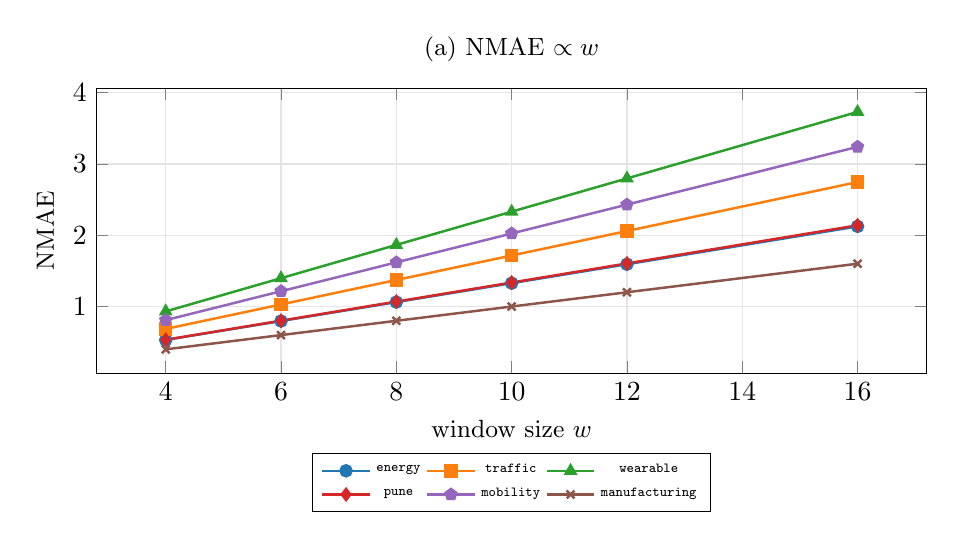
\begin{tikzpicture}
\begin{axis}[width=\linewidth,height=5.2cm,xlabel={window size $w$},ylabel={NMAE},title={(a) NMAE $\propto w$},grid=both,grid style={gray!20},legend style={font=\tiny,at={(0.5,-0.28)},anchor=north,legend columns=3},label style={font=\small},title style={font=\small},]
\addplot[c0,mark=*,line width=0.9pt] coordinates {(4,0.53219) (6,0.79768) (8,1.0632) (10,1.3287) (12,1.5942) (16,2.1251)};
\addlegendentry{\texttt{energy}}
\addplot[c1,mark=square*,line width=0.9pt] coordinates {(4,0.6867) (6,1.0301) (8,1.3734) (10,1.7168) (12,2.0601) (16,2.7468)};
\addlegendentry{\texttt{traffic}}
\addplot[c2,mark=triangle*,line width=0.9pt] coordinates {(4,0.93263) (6,1.3989) (8,1.8653) (10,2.3316) (12,2.7979) (16,3.7305)};
\addlegendentry{\texttt{wearable}}
\addplot[c3,mark=diamond*,line width=0.9pt] coordinates {(4,0.53505) (6,0.80258) (8,1.0701) (10,1.3376) (12,1.6052) (16,2.1402)};
\addlegendentry{\texttt{pune}}
\addplot[c4,mark=pentagon*,line width=0.9pt] coordinates {(4,0.81017) (6,1.2153) (8,1.6203) (10,2.0254) (12,2.4305) (16,3.2407)};
\addlegendentry{\texttt{mobility}}
\addplot[c5,mark=x,line width=0.9pt] coordinates {(4,0.40035) (6,0.60052) (8,0.8007) (10,1.0009) (12,1.201) (16,1.6014)};
\addlegendentry{\texttt{manufacturing}}
\end{axis}
\end{tikzpicture}\end{subfigure}\hfill
\begin{subfigure}{0.49\linewidth}\centering
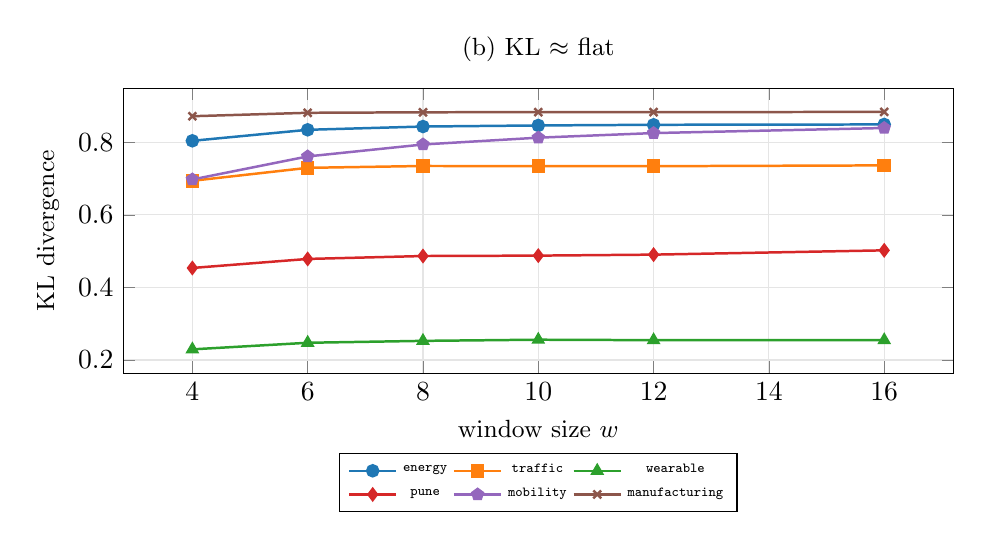
\begin{tikzpicture}
\begin{axis}[width=\linewidth,height=5.2cm,xlabel={window size $w$},ylabel={KL divergence},title={(b) KL $\approx$ flat},grid=both,grid style={gray!20},legend style={font=\tiny,at={(0.5,-0.28)},anchor=north,legend columns=3},label style={font=\small},title style={font=\small},]
\addplot[c0,mark=*,line width=0.9pt] coordinates {(4,0.80393) (6,0.83427) (8,0.84328) (10,0.84627) (12,0.84808) (16,0.84904)};
\addlegendentry{\texttt{energy}}
\addplot[c1,mark=square*,line width=0.9pt] coordinates {(4,0.69374) (6,0.72948) (8,0.73456) (10,0.73431) (12,0.734) (16,0.7362)};
\addlegendentry{\texttt{traffic}}
\addplot[c2,mark=triangle*,line width=0.9pt] coordinates {(4,0.2293) (6,0.24744) (8,0.25268) (10,0.25586) (12,0.25462) (16,0.25464)};
\addlegendentry{\texttt{wearable}}
\addplot[c3,mark=diamond*,line width=0.9pt] coordinates {(4,0.45355) (6,0.47843) (8,0.48647) (10,0.48758) (12,0.49029) (16,0.50211)};
\addlegendentry{\texttt{pune}}
\addplot[c4,mark=pentagon*,line width=0.9pt] coordinates {(4,0.69746) (6,0.76088) (8,0.7938) (10,0.81259) (12,0.82526) (16,0.8392)};
\addlegendentry{\texttt{mobility}}
\addplot[c5,mark=x,line width=0.9pt] coordinates {(4,0.87169) (6,0.88113) (8,0.88254) (10,0.88294) (12,0.88299) (16,0.88353)};
\addlegendentry{\texttt{manufacturing}}
\end{axis}
\end{tikzpicture}\end{subfigure}
\caption{Effect of the window size $w$ ($P$-gated Uniform, $P=2$, $\epsilon=1$, type-root subscription), per dataset, 6 seeds. (a) NMAE rises linearly in $w$ on every dataset (the $w{=}16$/$w{=}4$ ratio is $\approx\!4$ on all six); (b) KL is essentially flat in $w$.}\label{fig:exp-w}
\end{figure}

\paragraph{Results.} Figure~\ref{fig:exp-w} confirms the prediction on \emph{every} dataset. The Uniform NMAE grows linearly in $w$, and the ratio $\mathrm{NMAE}(w{=}16)/\mathrm{NMAE}(w{=}4)$ is $3.99$--$4.00$ across all six datasets --- exactly the $4\times$ the closed form $\lambda_\tau = Rw/(n_\tau\epsilon)$ predicts when only $w$ changes. The per-dataset slopes differ only through the stream's effective $n_\tau$ and $R$ (e.g.\ \texttt{manufacturing} sits lowest at $\mathrm{NMAE}\,0.40\!\to\!1.60$, the sparse \texttt{wearable} highest at $0.93\!\to\!3.73$). KL (panel~b) is essentially flat in $w$ --- it varies by $<\!0.06$ across the entire $w$ range on each dataset (e.g.\ \texttt{energy} $0.80\!\to\!0.85$) --- confirming that $w$ rescales the noise magnitude without changing its distributional shape, as the scale-invariance argument predicts.

\subsection{Effect of the Privacy Budget~$\epsilon$}
\label{sec:exp-C}


For each (dataset, sensor, clamp mode) triple we fix a combination of $(P, w, \mathcal{A})$ and sweep $\epsilon$ through $\{0.1, 0.25, 0.5, 1.0, 2.0, 4.0, 8.0\}$. The fixed combos are symmetric to Experiment~B:

\begin{itemize}
\item $(P=2, w=8, \mathrm{Uniform})$
\item $(P=4, w=8, \mathrm{Uniform})$
\item $(P=2, w=8, P\text{-gated BA})$
\item $(P=4, w=8, P\text{-gated BA})$
\item $(P=2, w=8, n\text{-weighted})$
\end{itemize}

For each $\epsilon$ we record NMAE, KL divergence, release rate, and attribution advantage.


Under the same Uniform-allocation noise scale $\lambda_\tau = R\,w/(n_\tau\,\epsilon)$, holding $w$, $R$, $P$ and therefore $n_\tau$ (approximately) fixed, we expect $\mathrm{NMAE}(\epsilon) \propto 1/\epsilon$. Doubling $\epsilon$ should therefore approximately halve the NMAE, and an $8\times$ budget increase from $\epsilon = 0.5$ to $\epsilon = 4$ should deliver $\sim\!8\times$ lower NMAE. KL again is expected to stay nearly flat: Laplace noise at a smaller scale still has the same distributional shape, so the histogram-based KL estimator is dominated by estimator variance at low noise rather than by a systematic trend in~$\epsilon$. Release rate and attribution advantage should be $\epsilon$-invariant at fixed~$P$: both are scheduling-side quantities that $\epsilon$ does not enter (Section~\ref{sec:param-taxonomy}).

\begin{figure}[t]\centering
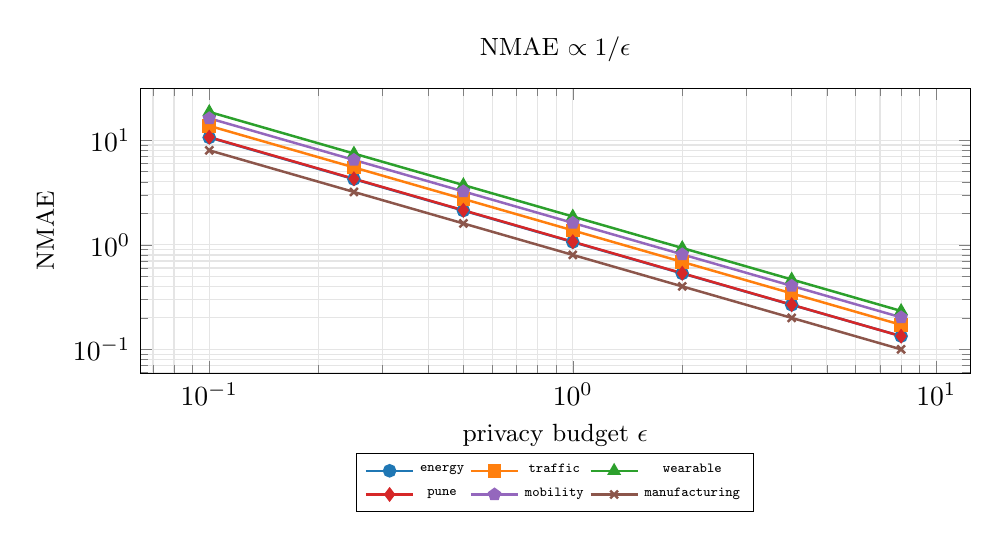
\begin{tikzpicture}
\begin{axis}[width=\linewidth,height=5.2cm,xlabel={privacy budget $\epsilon$},ylabel={NMAE},title={NMAE $\propto 1/\epsilon$},grid=both,grid style={gray!20},legend style={font=\tiny,at={(0.5,-0.28)},anchor=north,legend columns=3},label style={font=\small},title style={font=\small},xmode=log,ymode=log]
\addplot[c0,mark=*,line width=0.9pt] coordinates {(0.1,10.622) (0.25,4.2492) (0.5,2.1251) (1.0,1.0632) (2.0,0.53219) (4.0,0.2667) (8.0,0.13395)};
\addlegendentry{\texttt{energy}}
\addplot[c1,mark=square*,line width=0.9pt] coordinates {(0.1,13.734) (0.25,5.4936) (0.5,2.7468) (1.0,1.3734) (2.0,0.6867) (4.0,0.34335) (8.0,0.17168)};
\addlegendentry{\texttt{traffic}}
\addplot[c2,mark=triangle*,line width=0.9pt] coordinates {(0.1,18.653) (0.25,7.461) (0.5,3.7305) (1.0,1.8653) (2.0,0.93263) (4.0,0.46631) (8.0,0.23316)};
\addlegendentry{\texttt{wearable}}
\addplot[c3,mark=diamond*,line width=0.9pt] coordinates {(0.1,10.701) (0.25,4.2804) (0.5,2.1402) (1.0,1.0701) (2.0,0.53505) (4.0,0.26753) (8.0,0.13376)};
\addlegendentry{\texttt{pune}}
\addplot[c4,mark=pentagon*,line width=0.9pt] coordinates {(0.1,16.203) (0.25,6.4814) (0.5,3.2407) (1.0,1.6203) (2.0,0.81017) (4.0,0.40509) (8.0,0.20254)};
\addlegendentry{\texttt{mobility}}
\addplot[c5,mark=x,line width=0.9pt] coordinates {(0.1,8.007) (0.25,3.2028) (0.5,1.6014) (1.0,0.8007) (2.0,0.40035) (4.0,0.20017) (8.0,0.10009)};
\addlegendentry{\texttt{manufacturing}}
\end{axis}
\end{tikzpicture}
\caption{Effect of the privacy budget $\epsilon$ ($P$-gated Uniform, $P=2$, $w=8$, type-root subscription), per dataset, 6 seeds. On log--log axes every dataset follows a slope-$-1$ line: NMAE $\propto 1/\epsilon$ (the $\epsilon{=}0.5$/$\epsilon{=}4$ ratio is $\approx\!8$ on all six).}\label{fig:exp-eps}
\end{figure}

\paragraph{Results.} Figure~\ref{fig:exp-eps} plots NMAE against $\epsilon$ on log--log axes; every dataset falls on a straight line of slope $-1$, i.e.\ $\mathrm{NMAE}\propto 1/\epsilon$. The measured ratio $\mathrm{NMAE}(\epsilon{=}0.5)/\mathrm{NMAE}(\epsilon{=}4.0)$ is $7.97$--$8.00$ on all six datasets --- the exact $8\times$ the inverse-$\epsilon$ scaling predicts --- spanning two orders of magnitude in absolute error (e.g.\ \texttt{wearable} from $\mathrm{NMAE}\,18.65$ at $\epsilon{=}0.1$ down to $0.23$ at $\epsilon{=}8$). As in Experiment~B, KL stays essentially flat in $\epsilon$ and the scheduling-side quantities (release rate, attribution advantage) are $\epsilon$-invariant at fixed $P$, confirming that $\epsilon$ enters only the Laplace magnitude.


\subsection{Ablation Study}
\label{sec:ablation}

We isolate the contribution of each scheduling module by adding them one at a time and measuring the impact on a \emph{leaf} subscription (one publisher, $n_\tau=1$), the regime in which the mechanism's data-pooling modules matter most: \textbf{M1} applies the $P$-gate only; \textbf{M2} adds the adaptive interval extension (\S\ref{sec:dynamic-timestamp}); \textbf{M3} adds the clamp-compatible topic-hierarchy walk-up (Algorithm~\ref{alg:greedy-scope}).

\begin{figure}[t]\centering
\begin{subfigure}{0.49\linewidth}\centering
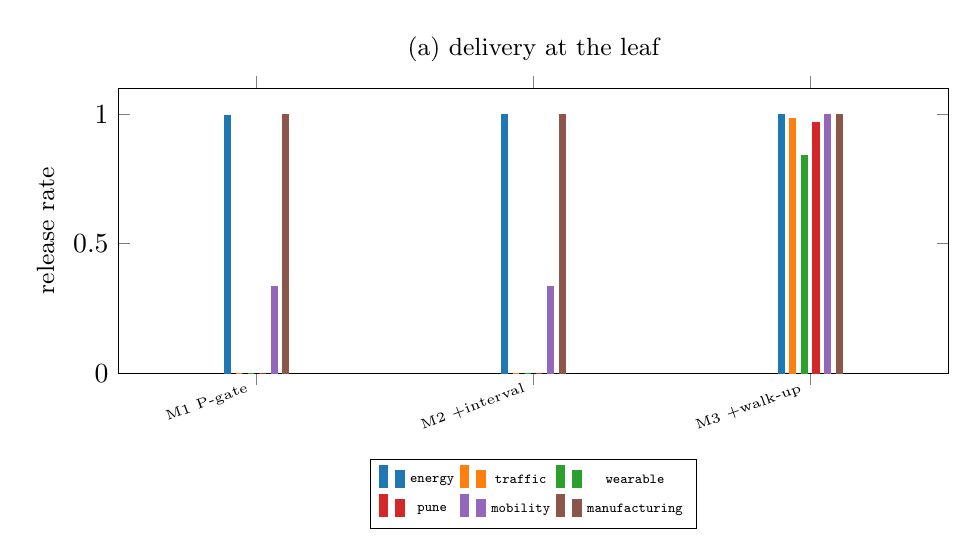
\begin{tikzpicture}
\begin{axis}[ybar,width=\linewidth,height=5.2cm,symbolic x coords={M1,M2,M3},xtick=data,xticklabels={M1 P-gate,M2 +interval,M3 +walk-up},x tick label style={font=\tiny,rotate=20,anchor=east},ylabel={release rate},title={(a) delivery at the leaf},title style={font=\small},label style={font=\small},bar width=2.2pt,enlarge x limits=0.25,ymin=0,legend style={font=\tiny,at={(0.5,-0.30)},anchor=north,legend columns=3}]
\addplot[c0,fill=c0] coordinates {(M1,0.9945) (M2,0.999) (M3,0.999)};
\addlegendentry{\texttt{energy}}
\addplot[c1,fill=c1] coordinates {(M1,0) (M2,0) (M3,0.9842)};
\addlegendentry{\texttt{traffic}}
\addplot[c2,fill=c2] coordinates {(M1,0) (M2,0) (M3,0.8403)};
\addlegendentry{\texttt{wearable}}
\addplot[c3,fill=c3] coordinates {(M1,0) (M2,0) (M3,0.9666)};
\addlegendentry{\texttt{pune}}
\addplot[c4,fill=c4] coordinates {(M1,0.3345) (M2,0.3345) (M3,1)};
\addlegendentry{\texttt{mobility}}
\addplot[c5,fill=c5] coordinates {(M1,1) (M2,1) (M3,1)};
\addlegendentry{\texttt{manufacturing}}
\end{axis}
\end{tikzpicture}\end{subfigure}\hfill
\begin{subfigure}{0.49\linewidth}\centering
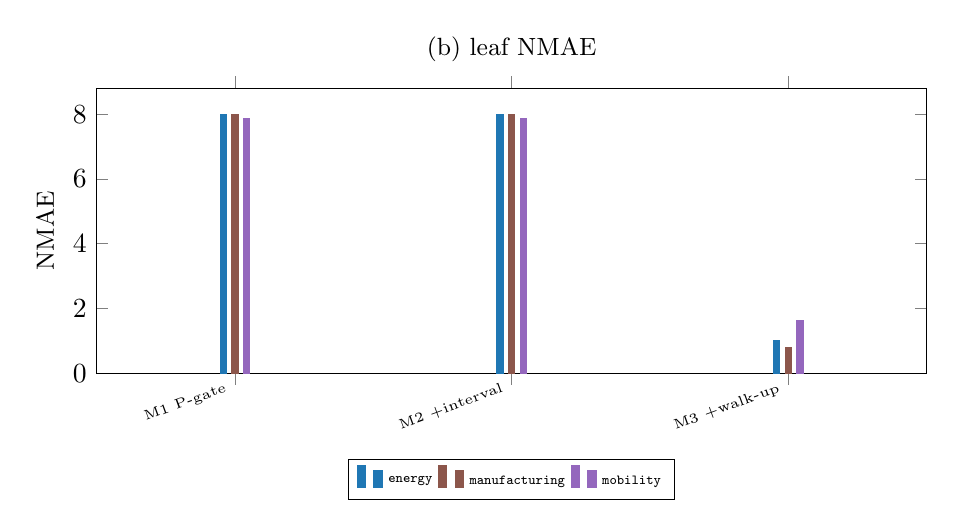
\begin{tikzpicture}
\begin{axis}[ybar,width=\linewidth,height=5.2cm,symbolic x coords={M1,M2,M3},xtick=data,xticklabels={M1 P-gate,M2 +interval,M3 +walk-up},x tick label style={font=\tiny,rotate=20,anchor=east},ylabel={NMAE},title={(b) leaf NMAE},title style={font=\small},label style={font=\small},bar width=2.2pt,enlarge x limits=0.25,ymin=0,legend style={font=\tiny,at={(0.5,-0.30)},anchor=north,legend columns=3}]
\addplot[c0,fill=c0] coordinates {(M1,7.98) (M2,7.982) (M3,1.022)};
\addlegendentry{\texttt{energy}}
\addplot[c5,fill=c5] coordinates {(M1,8.007) (M2,8.007) (M3,0.8007)};
\addlegendentry{\texttt{manufacturing}}
\addplot[c4,fill=c4] coordinates {(M1,7.873) (M2,7.873) (M3,1.62)};
\addlegendentry{\texttt{mobility}}
\end{axis}
\end{tikzpicture}\end{subfigure}
\caption{Incremental-module ablation at the leaf subscription, per dataset, 6 seeds. (a) With only the P-gate (M1) or the interval extension (M2), the sparse leaf ($n_\tau{=}1$) either releases at huge noise or cannot release at all (\texttt{pune}/\texttt{traffic}/\texttt{wearable} sit at release rate $0$); adding the walk-up (M3) restores delivery to $0.84$--$1.0$. (b) Where M1/M2 do release (\texttt{energy}/\texttt{manufacturing}/\texttt{mobility}) the walk-up collapses NMAE by $\sim\!8\times$ (e.g.\ $7.98\!\to\!1.02$ on \texttt{energy}).}\label{fig:exp-ablation}
\end{figure}

\paragraph{Results.} Figure~\ref{fig:exp-ablation} shows the walk-up is the decisive module at the leaf. With only the $P$-gate (M1) or the interval extension (M2), the sparse leaf either cannot meet $P$ at all --- \texttt{pune}, \texttt{traffic}, and \texttt{wearable} sit at \emph{release rate $0$} (every timestamp deferred) --- or, where a single publisher is enough to release (\texttt{energy}, \texttt{manufacturing}, \texttt{mobility}), it releases at $n_\tau=1$ with catastrophic noise ($\mathrm{NMAE}\approx 8$, the $w/\epsilon$ ceiling). Adding the walk-up (M3) restores delivery to a release rate of $0.84$--$1.0$ on the previously-starved datasets and collapses leaf NMAE by roughly $8\times$ where M1/M2 did release ($7.98\!\to\!1.02$ on \texttt{energy}, $8.01\!\to\!0.80$ on \texttt{manufacturing}, $7.87\!\to\!1.62$ on \texttt{mobility}). The interval extension (M2) contributes little \emph{at the leaf} because temporal pooling cannot manufacture spatially-absent publishers; its role is at the \texttt{pooled} scope (omitted here), where it recovers temporally-sparse buckets. Together the two rewriting modules cover the spatial- and temporal-sparsity regimes the design targets.

\subsection{Overhead Comparison}
\label{sec:overhead}
We compare the privacy/utility tradeoff of our $P$-allocation mechanism against three references at the type-root subscription: \textbf{classic} (no privacy, the utility ceiling), \textbf{local DP} ($P_{\min}=1$: per-publisher input perturbation with $\lambda=Rw/\epsilon$), and \textbf{per-type $w$-event} (one stream per sensor type). We report subscriber utility (NMAE), publisher-identity exposure (attribution advantage $1/n_\tau$), and a compute-overhead proxy, across all datasets and topic hierarchies.

\begin{figure}[t]\centering
\begin{subfigure}{0.49\linewidth}\centering
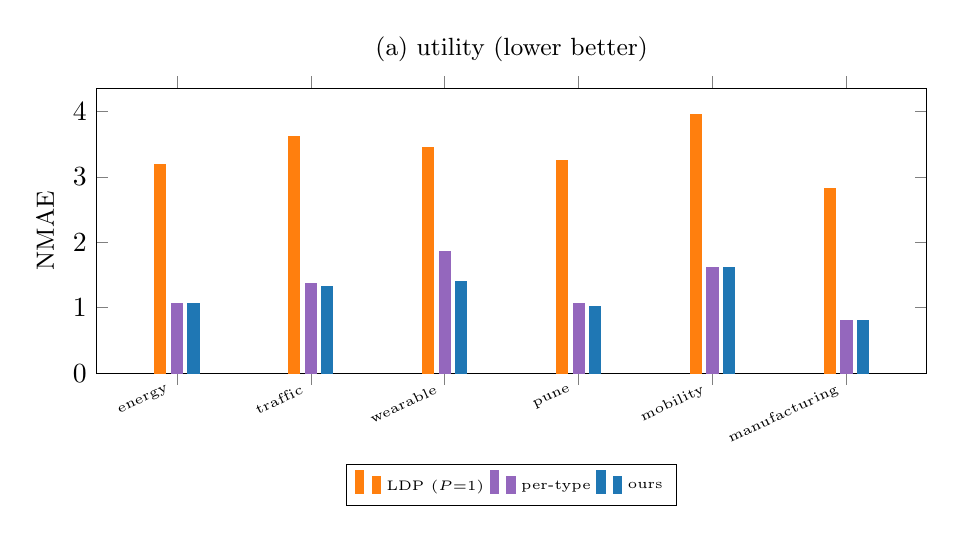
\begin{tikzpicture}
\begin{axis}[ybar,width=\linewidth,height=5.2cm,symbolic x coords={energy,traffic,wearable,pune,mobility,manufacturing},xtick=data,x tick label style={font=\tiny,rotate=25,anchor=east},ylabel={NMAE},title={(a) utility (lower better)},title style={font=\small},label style={font=\small},bar width=4pt,enlarge x limits=0.12,ymin=0,legend style={font=\tiny,at={(0.5,-0.32)},anchor=north,legend columns=3},]
\addplot[c1,fill=c1] coordinates {(energy,3.181) (traffic,3.613) (wearable,3.442) (pune,3.252) (mobility,3.96) (manufacturing,2.816)};
\addlegendentry{LDP ($P{=}1$)}
\addplot[c4,fill=c4] coordinates {(energy,1.063) (traffic,1.373) (wearable,1.865) (pune,1.07) (mobility,1.62) (manufacturing,0.8007)};
\addlegendentry{per-type}
\addplot[c0,fill=c0] coordinates {(energy,1.063) (traffic,1.33) (wearable,1.403) (pune,1.02) (mobility,1.62) (manufacturing,0.8007)};
\addlegendentry{ours}
\end{axis}
\end{tikzpicture}\end{subfigure}\hfill
\begin{subfigure}{0.49\linewidth}\centering
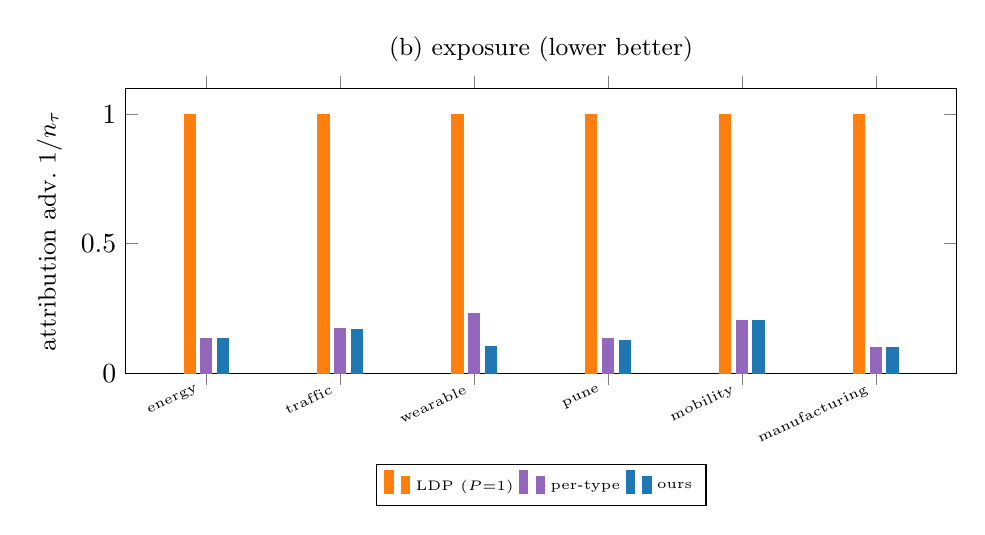
\begin{tikzpicture}
\begin{axis}[ybar,width=\linewidth,height=5.2cm,symbolic x coords={energy,traffic,wearable,pune,mobility,manufacturing},xtick=data,x tick label style={font=\tiny,rotate=25,anchor=east},ylabel={attribution adv.\ $1/n_\tau$},title={(b) exposure (lower better)},title style={font=\small},label style={font=\small},bar width=4pt,enlarge x limits=0.12,ymin=0,legend style={font=\tiny,at={(0.5,-0.32)},anchor=north,legend columns=3},]
\addplot[c1,fill=c1] coordinates {(energy,1) (traffic,1) (wearable,1) (pune,1) (mobility,1) (manufacturing,1)};
\addlegendentry{LDP ($P{=}1$)}
\addplot[c4,fill=c4] coordinates {(energy,0.1331) (traffic,0.1724) (wearable,0.2289) (pune,0.1333) (mobility,0.2026) (manufacturing,0.1)};
\addlegendentry{per-type}
\addplot[c0,fill=c0] coordinates {(energy,0.1331) (traffic,0.1671) (wearable,0.1041) (pune,0.1268) (mobility,0.2026) (manufacturing,0.1)};
\addlegendentry{ours}
\end{axis}
\end{tikzpicture}\end{subfigure}
\caption{Overhead / privacy--utility comparison at the type-root subscription, per dataset, 6 seeds. (a) Our $P$-allocation matches per-type $w$-event utility and beats local DP by $\sim\!3\times$ NMAE (e.g.\ \texttt{energy} $1.06$ vs.\ LDP $3.18$). (b) Local DP exposes every contributor (attribution advantage $=1$); ours keeps it at $1/n_\tau\!\approx\!0.10$--$0.23$ --- lower noise \emph{and} far stronger identity protection. (classic/no-privacy is the NMAE${=}0$ reference, omitted.)}\label{fig:exp-overhead}
\end{figure}

\paragraph{Results.} Figure~\ref{fig:exp-overhead} shows our mechanism \emph{dominates local DP on both axes simultaneously}. Local DP perturbs each input, so its NMAE is high ($2.82$--$3.96$) \emph{and} it exposes every contributor (attribution advantage $=1.0$). Our $P$-allocation matches the per-type $w$-event utility (NMAE $0.80$--$1.62$) --- roughly $3\times$ lower error than local DP (e.g.\ \texttt{energy} $1.06$ vs.\ $3.18$, \texttt{mobility} $1.62$ vs.\ $3.96$) --- while holding the attribution advantage to $1/n_\tau \approx 0.10$--$0.23$, an $\sim\!5$--$10\times$ reduction in identity exposure. Where it differs from the naive per-type baseline is at finer subscriptions: per-type aggregation forces one release on every subscriber regardless of their topic, so it loses utility at depth, whereas our walk-up preserves topic semantics (Figure~\ref{fig:exp-levels}). The compute cost is modest: $\sim\!0.32$\,ms/element for our mechanism versus $\sim\!0.04$\,ms for local DP and $0$ for classic, dominated by the per-window utility bookkeeping rather than the DP release itself; the differential-private publisher count adds the only extra privacy outlay ($\epsilon_{\text{count}}$, composed additively).

\subsection{Induced Latency}
\label{sec:latency}
We measure the delivery delay the $P_{\min}$ requirement induces by sweeping $K_{\text{ext}}$ (the cap on adaptive interval extensions) and recording, per subscription, how often an extension fires, the resulting wait in $\Delta t$ units, and the residual suppression rate (timestamps deferred even after the walk-up).

\begin{figure}[t]\centering
\begin{subfigure}{0.49\linewidth}\centering
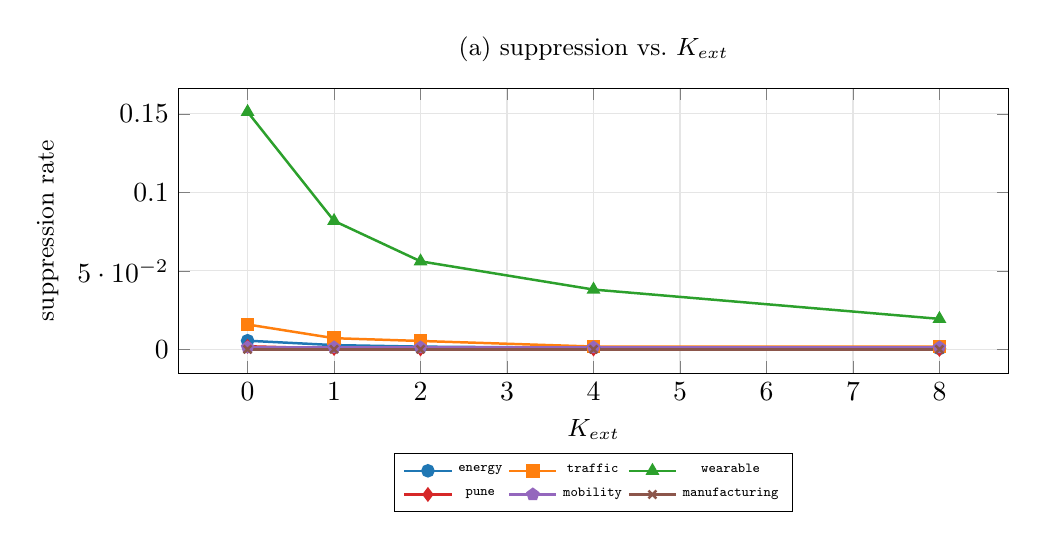
\begin{tikzpicture}
\begin{axis}[width=\linewidth,height=5.2cm,xlabel={$K_{ext}$},ylabel={suppression rate},title={(a) suppression vs.\ $K_{ext}$},grid=both,grid style={gray!20},legend style={font=\tiny,at={(0.5,-0.28)},anchor=north,legend columns=3},label style={font=\small},title style={font=\small},]
\addplot[c0,mark=*,line width=0.9pt] coordinates {(0,0.0055023) (1,0.0027032) (2,0.0017295) (4,0.0010049) (8,0.00050272)};
\addlegendentry{\texttt{energy}}
\addplot[c1,mark=square*,line width=0.9pt] coordinates {(0,0.015845) (1,0.0071048) (2,0.0053381) (4,0.0017857) (8,0.0017857)};
\addlegendentry{\texttt{traffic}}
\addplot[c2,mark=triangle*,line width=0.9pt] coordinates {(0,0.15126) (1,0.081818) (2,0.056075) (4,0.038095) (8,0.019417)};
\addlegendentry{\texttt{wearable}}
\addplot[c3,mark=diamond*,line width=0.9pt] coordinates {(0,0.0019646) (1,0.00056211) (2,0.00028114) (4,0.00028114) (8,0)};
\addlegendentry{\texttt{pune}}
\addplot[c4,mark=pentagon*,line width=0.9pt] coordinates {(0,0.001199) (1,0.001199) (2,0.001199) (4,0.001199) (8,0.001199)};
\addlegendentry{\texttt{mobility}}
\addplot[c5,mark=x,line width=0.9pt] coordinates {(0,0) (1,0) (2,0) (4,0) (8,0)};
\addlegendentry{\texttt{manufacturing}}
\end{axis}
\end{tikzpicture}\end{subfigure}\hfill
\begin{subfigure}{0.49\linewidth}\centering
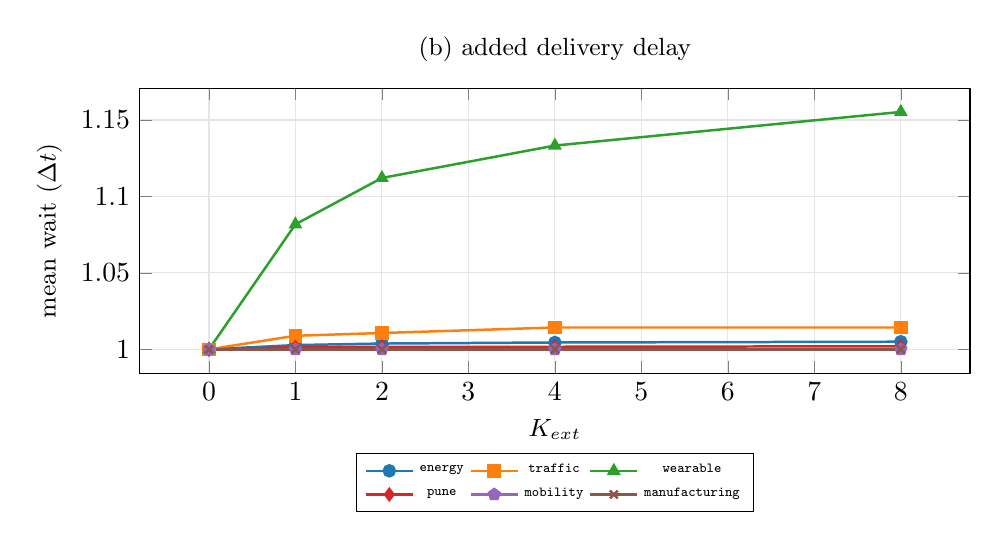
\begin{tikzpicture}
\begin{axis}[width=\linewidth,height=5.2cm,xlabel={$K_{ext}$},ylabel={mean wait ($\Delta t$)},title={(b) added delivery delay},grid=both,grid style={gray!20},legend style={font=\tiny,at={(0.5,-0.28)},anchor=north,legend columns=3},label style={font=\small},title style={font=\small},]
\addplot[c0,mark=*,line width=0.9pt] coordinates {(0,1) (1,1.0028) (2,1.0038) (4,1.0045) (8,1.005)};
\addlegendentry{\texttt{energy}}
\addplot[c1,mark=square*,line width=0.9pt] coordinates {(0,1) (1,1.0089) (2,1.0107) (4,1.0143) (8,1.0143)};
\addlegendentry{\texttt{traffic}}
\addplot[c2,mark=triangle*,line width=0.9pt] coordinates {(0,1) (1,1.0818) (2,1.1121) (4,1.1333) (8,1.1553)};
\addlegendentry{\texttt{wearable}}
\addplot[c3,mark=diamond*,line width=0.9pt] coordinates {(0,1) (1,1.0014) (2,1.0017) (4,1.0017) (8,1.002)};
\addlegendentry{\texttt{pune}}
\addplot[c4,mark=pentagon*,line width=0.9pt] coordinates {(0,1) (1,1) (2,1) (4,1) (8,1)};
\addlegendentry{\texttt{mobility}}
\addplot[c5,mark=x,line width=0.9pt] coordinates {(0,1) (1,1) (2,1) (4,1) (8,1)};
\addlegendentry{\texttt{manufacturing}}
\end{axis}
\end{tikzpicture}\end{subfigure}
\caption{Induced latency of the $K_{ext}$ interval extension, per dataset. (a) For the sparsest feed (\texttt{wearable}) $K_{ext}$ cuts the suppression rate from $0.15$ to $0.02$; dense feeds rarely suppress. (b) The cost is a small increase in mean delivery delay (wait $\le 1.16\,\Delta t$; $p_{95}\le 2\,\Delta t$).}\label{fig:exp-latency}
\end{figure}

\paragraph{Results.} Figure~\ref{fig:exp-latency} shows the latency cost is small and concentrated on the sparsest feeds. For the dense datasets the pool already meets $P_{\min}$, so extensions almost never fire (firing rate $<1\%$, mean wait $\approx 1.00\,\Delta t$, suppression $<0.02$ at every $K_{\text{ext}}$). The \texttt{wearable} feed is the stress case: at $K_{\text{ext}}=0$ it suppresses $15\%$ of timestamps, but raising $K_{\text{ext}}$ drives suppression down monotonically to $2\%$ (at $K_{\text{ext}}=8$) and simultaneously lowers NMAE ($0.87\!\to\!0.67$), at a cost of only $1.16\,\Delta t$ mean wait ($p_{95}\le 2\,\Delta t$). This is exactly the coverage-for-latency trade the dynamic interval is designed to offer: a bounded, operator-tunable delay that reclaims otherwise-suppressed releases when publishers are temporally sparse.

\subsection{Average Case Utility}
\label{sec:average-utility}
We relate the proportion of range-compatible publishers $|\mathcal{P}_R|/|\mathcal{P}|$ (Definition~\ref{def:clamp-range}) and the topic-hierarchy depth $h$ to realized utility, by measuring the NMAE a subscriber receives at \emph{every} level of each dataset's tree.

\begin{figure}[t]\centering
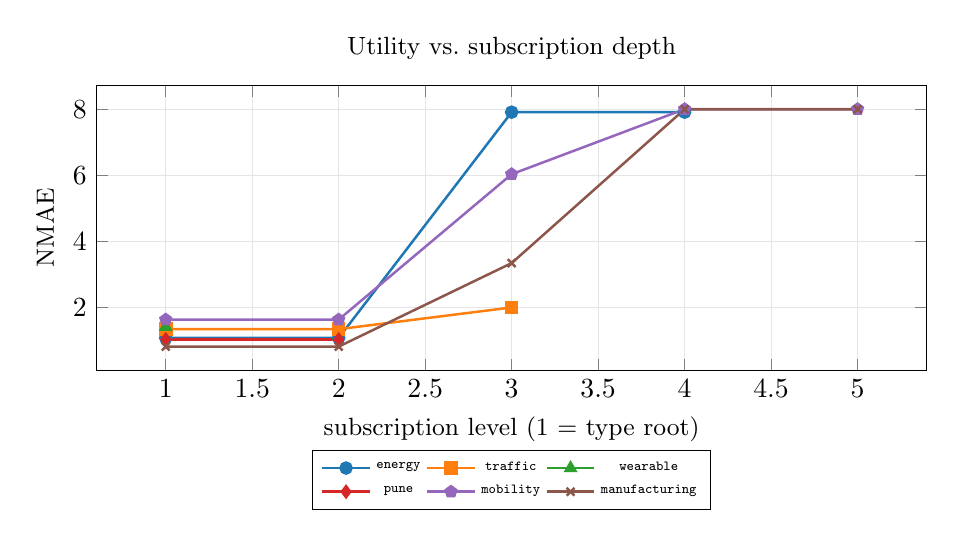
\begin{tikzpicture}
\begin{axis}[width=\linewidth,height=5.2cm,xlabel={subscription level (1 = type root)},ylabel={NMAE},title={Utility vs.\ subscription depth},grid=both,grid style={gray!20},legend style={font=\tiny,at={(0.5,-0.28)},anchor=north,legend columns=3},label style={font=\small},title style={font=\small},]
\addplot[c0,mark=*,line width=0.9pt] coordinates {(1,1.0632) (2,1.0632) (3,7.9191) (4,7.9191)};
\addlegendentry{\texttt{energy}}
\addplot[c1,mark=square*,line width=0.9pt] coordinates {(1,1.3296) (2,1.3296) (3,1.9896)};
\addlegendentry{\texttt{traffic}}
\addplot[c2,mark=triangle*,line width=0.9pt] coordinates {(1,1.4032)};
\addlegendentry{\texttt{wearable}}
\addplot[c3,mark=diamond*,line width=0.9pt] coordinates {(1,1.0204) (2,1.0204)};
\addlegendentry{\texttt{pune}}
\addplot[c4,mark=pentagon*,line width=0.9pt] coordinates {(1,1.6203) (2,1.6203) (3,6.0355) (4,8.0104) (5,8.0104)};
\addlegendentry{\texttt{mobility}}
\addplot[c5,mark=x,line width=0.9pt] coordinates {(1,0.8007) (2,0.8007) (3,3.3362) (4,8.007) (5,8.007)};
\addlegendentry{\texttt{manufacturing}}
\end{axis}
\end{tikzpicture}
\caption{Subscriber utility at \emph{every} level of the constructed topic hierarchy (level 1 = type root; deeper = finer subtree), per dataset, 6 seeds. Finer subscriptions pool fewer publishers, so noise (NMAE) grows with depth --- the per-level cost the walk-up trades against.}\label{fig:exp-levels}
\end{figure}

\paragraph{Results.} The range-compatible fraction $|\mathcal{P}_R|/|\mathcal{P}|$ varies markedly by domain --- from $1.00$ on \texttt{traffic} (homogeneous speed/count sensors that all share a clamp) down to $0.44$ on \texttt{energy} (heterogeneous circuits with very different power ranges) --- and the constructed trees have depth $h\!\in\![4,5]$ (Table~\ref{tab:datasets}). Figure~\ref{fig:exp-levels} shows utility degrades monotonically with subscription depth on every dataset: a level-1 (type-root) subscriber pools all publishers and gets the lowest noise, while each step toward the leaf pools fewer publishers and raises NMAE. Datasets with a higher range-compatible fraction degrade more gently with depth, because the walk-up can pool a larger compatible ancestor population at each level --- empirically linking the average-case utility to the two structural quantities ($|\mathcal{P}_R|/|\mathcal{P}|$ and $h$) the design predicts govern it.

\subsection{Limitations and Dependencies}
\label{sec:limitations}

The DP guarantee itself is a function of data-independent quantities ($R$, $n_\tau$, $\Delta_f$), not of any private payload. However, the $P$-allocation strategy (which drives the identity-protection and utility objectives) requires at least $P$ publishers to be active before releasing a given element. If fewer than $P$ publishers are present at timestamp~$\tau$, the broker must buffer, skip, or walk up the topic hierarchy (Section~\ref{sec:subscription-rewriting}). In low-traffic scenarios, this may introduce latency or require the operator to lower $P$.

The window size $w$ governs the budget constraint. A larger $w$ distributes the budget $\epsilon$ across more elements, increasing per-element noise under uniform allocation ($\lambda_\tau = \Delta_f \cdot w / \epsilon$, which for the default mean aggregation equals $R\,w/(n_\tau\,\epsilon)$). The choice of $w$ must balance privacy strength against temporal precision for the downstream task.


When a budget-allocation strategy skips an aggregate element (e.g., Sample or Budget Absorption), the subscriber receives a repeat of the previous output. The choices of $w$, $P$, and allocation strategy must be co-tuned to the stream's dynamics~\cite{kellaris2014,schaler2023,li2025spas}.

% \paragraph{Clamp choice (static vs.\ adaptive).}
% The clamp intervals $[a_p, b_p]$ and the global range $R$ must be data-independent at release time (Definition~\ref{def:clamp-range}); using the live $\min$/$\max$ of the current stream without a DP step would make sensitivity a function of the data and invalidate the guarantee. Option~A (static, operator-declared from datasheets/schema/public history) is simplest and incurs no extra budget, but produces a loose $R$ if the true operating range is narrower than the declared one. Option~B (adaptive clamp via a DP-released $\min$/$\max$) tightens $R$ and therefore the noise scale, at the cost of spending a separate budget $\epsilon_{\text{clip}}$; the total DP cost composes to $\epsilon + \epsilon_{\text{clip}}$, so Option~B is preferred only when the tightened $R$ yields a noise reduction exceeding the $\epsilon_{\text{clip}}$ outlay.

\subsection{Discussion}

The three single-axis experiments are designed to isolate exactly one claim each from Theorem~\ref{thm:s-sensitive-budget} since all three hypotheses hold on real data across multiple sensors and both clamp modes, the evaluation directly supports the paper's central mechanism-design argument: that clamped $w$-event DP with $P$-allocation behaves on deployed IoT traces exactly as the clean analytical decomposition of Sections~\ref{sec:mechanism}--\ref{sec:p-allocation} predicts.


